\appendix
\chapter{Anexo I: Historias de usuario}\label{cap:anexo1}

En este anexo se presentan el resto de las historias de usuario identificadas durante el desarrollo del proyecto. Estas historias describen funcionalidades adicionales que permiten expandir las capacidades del sistema, garantizando una plataforma más completa y eficiente. A continuación, se encuentran detalladas con sus respectivas descripciones, criterios de validación, prioridades, estimaciones y dependencias.

\vspace{0.5cm}

\begin{table}[H]
  \centering
  \renewcommand{\arraystretch}{1.5}
  \begin{tabular}{|p{0.3\textwidth}|p{0.3\textwidth}|p{0.3\textwidth}|}
    \hline
    \multicolumn{3}{|l|}{\cellcolor{OrangeVIU}\textcolor{white}{\textbf{(H3) Historia de usuario 3: Formulario de registro}}} \\
    \hline
    \multicolumn{3}{|p{\dimexpr0.9\linewidth+2\tabcolsep+2\arrayrulewidth}|}{{\textbf{\textcolor{naranja}{Descripción: }}}Desarrollar un formulario de registro que permita a los usuarios crear una cuenta en el sistema proporcionando información básica como nombre, dirección de correo electrónico y contraseña.} \\
    \hline
    \multicolumn{3}{|p{\dimexpr0.9\linewidth+2\tabcolsep+2\arrayrulewidth}|}{{\textbf{\textcolor{naranja}{Validación: }} Verificar que el formulario de registro esté correctamente implementado y sea accesible desde la interfaz de usuario.}} \\
    \hline
    {\textbf{\textcolor{naranja}{Prioridad }}}  & {\textbf{\textcolor{naranja}{Estimación }}}  & {\textbf{\textcolor{naranja}{Dependencia }}}  \\
    \hline
    1 &  10h &  1 \\
    \hline
  \end{tabular}
  \caption{(H3) Historia de usuario 3 - Formulario de registro}
  \label{table:H3}
\end{table}


\begin{table}[H]
  \centering
  \renewcommand{\arraystretch}{1.5}
  \begin{tabular}{|p{0.3\textwidth}|p{0.3\textwidth}|p{0.3\textwidth}|}
    \hline
    \multicolumn{3}{|l|}{\cellcolor{OrangeVIU}\textcolor{white}{\textbf{(H4) Historia de usuario 4: Login de usuario}}} \\
    \hline
    \multicolumn{3}{|p{\dimexpr0.9\linewidth+2\tabcolsep+2\arrayrulewidth}|}{{\textbf{\textcolor{naranja}{Descripción: }}}Implementar un sistema de inicio de sesión que permita a los usuarios autenticarse en el sistema utilizando sus credenciales registradas.} \\
    \hline
    \multicolumn{3}{|p{\dimexpr0.9\linewidth+2\tabcolsep+2\arrayrulewidth}|}{{\textbf{\textcolor{naranja}{Validación: }} Confirmar que los usuarios puedan iniciar sesión utilizando su dirección de correo electrónico y contraseña.}} \\
    \hline
    {\textbf{\textcolor{naranja}{Prioridad }}}  & {\textbf{\textcolor{naranja}{Estimación }}}  & {\textbf{\textcolor{naranja}{Dependencia }}}  \\
    \hline
    1 &  15h &  1, 3 \\
    \hline
  \end{tabular}
  \caption{(H4) Historia de usuario 4 - Login de usuario}
  \label{table:H4}
\end{table}

\begin{table}[H]
  \centering
  \renewcommand{\arraystretch}{1.5}
  \begin{tabular}{|p{0.3\textwidth}|p{0.3\textwidth}|p{0.3\textwidth}|}
    \hline
    \multicolumn{3}{|l|}{\cellcolor{OrangeVIU}\textcolor{white}{\textbf{(H5) Historia de usuario 5: Diferenciación entre usuarios}}} \\
    \hline
    \multicolumn{3}{|p{\dimexpr0.9\linewidth+2\tabcolsep+2\arrayrulewidth}|}{{\textbf{\textcolor{naranja}{Descripción: }}}Desarrollar una funcionalidad que permita diferenciar entre usuarios administradores y usuarios regulares en el sistema, asignando roles y permisos específicos a cada tipo de usuario.} \\
    \hline
    \multicolumn{3}{|p{\dimexpr0.9\linewidth+2\tabcolsep+2\arrayrulewidth}|}{{\textbf{\textcolor{naranja}{Validación: }} Verificar que el sistema identifique correctamente a los usuarios administradores y usuarios regulares durante el proceso de autenticación.}} \\
    \hline
    {\textbf{\textcolor{naranja}{Prioridad }}}  & {\textbf{\textcolor{naranja}{Estimación }}}  & {\textbf{\textcolor{naranja}{Dependencia }}}  \\
    \hline
    1 &  10h &  1, 3, 4  \\
    \hline
  \end{tabular}
  \caption{(H5) Historia de usuario 5 - Diferenciación entre usuarios}
  \label{table:H5}
\end{table}

\begin{table}[H]
  \centering
  \renewcommand{\arraystretch}{1.5}
  \begin{tabular}{|p{0.3\textwidth}|p{0.3\textwidth}|p{0.3\textwidth}|}
    \hline
    \multicolumn{3}{|l|}{\cellcolor{OrangeVIU}\textcolor{white}{\textbf{(H6) Historia de usuario 6: Gestión de productos}}} \\
    \hline
    \multicolumn{3}{|p{\dimexpr0.9\linewidth+2\tabcolsep+2\arrayrulewidth}|}{{\textbf{\textcolor{naranja}{Descripción: }}}Permitir a los administradores gestionar los productos, incluyendo la capacidad de clasificarlos en categorías, editarlos, eliminarlos, agregar imágenes y otros detalles relevantes como precio y descripción.} \\
    \hline
    \multicolumn{3}{|p{\dimexpr0.9\linewidth+2\tabcolsep+2\arrayrulewidth}|}{{\textbf{\textcolor{naranja}{Validación: }} Verificar que los productos puedan ser gestionados correctamente, comprobando que se puedan clasificar en categorías, editar detalles, eliminar productos y agregar imágenes. }} \\
    \hline
    {\textbf{\textcolor{naranja}{Prioridad }}}  & {\textbf{\textcolor{naranja}{Estimación }}}  & {\textbf{\textcolor{naranja}{Dependencia }}}  \\
    \hline
    1 &  30h &  1, 2 \\
    \hline
  \end{tabular}
  \caption{(H6) Historia de usuario 6 - Gestión de productos}
  \label{table:H6}
\end{table}

\begin{table}[H]
  \centering
  \renewcommand{\arraystretch}{1.5}
  \begin{tabular}{|p{0.3\textwidth}|p{0.3\textwidth}|p{0.3\textwidth}|}
    \hline
    \multicolumn{3}{|l|}{\cellcolor{OrangeVIU}\textcolor{white}{\textbf{(H7) Historia de usuario 7: Mostrar productos}}} \\
    \hline
    \multicolumn{3}{|p{\dimexpr0.9\linewidth+2\tabcolsep+2\arrayrulewidth}|}{{\textbf{\textcolor{naranja}{Descripción: }}}Implementar una funcionalidad que permita a los usuarios visualizar los productos disponibles en el sistema, organizados por categorías. Cada producto mostrará información relevante como nombre, descripción, precio e imágenes, facilitando la navegación por las distintas categorías.} \\
    \hline
    \multicolumn{3}{|p{\dimexpr0.9\linewidth+2\tabcolsep+2\arrayrulewidth}|}{{\textbf{\textcolor{naranja}{Validación: }}  Verificar que los productos se muestren correctamente en sus respectivas categorías, garantizando que la interfaz sea clara, accesible y que toda la información esencial de cada producto esté disponible para el usuario de manera intuitiva.}} \\
    \hline
    {\textbf{\textcolor{naranja}{Prioridad }}}  & {\textbf{\textcolor{naranja}{Estimación }}}  & {\textbf{\textcolor{naranja}{Dependencia }}}  \\
    \hline
    1 &  20h &  1, 2, 6 \\
    \hline
  \end{tabular}
  \caption{(H7) Historia de usuario 7 - Mostrar productos}
  \label{table:H7}
\end{table}

\begin{table}[H]
  \centering
  \renewcommand{\arraystretch}{1.5}
  \begin{tabular}{|p{0.3\textwidth}|p{0.3\textwidth}|p{0.3\textwidth}|}
    \hline
    \multicolumn{3}{|l|}{\cellcolor{OrangeVIU}\textcolor{white}{\textbf{(H8) Historia de usuario 8: Venta en línea de productos}}} \\
    \hline
    \multicolumn{3}{|p{\dimexpr0.9\linewidth+2\tabcolsep+2\arrayrulewidth}|}{{\textbf{\textcolor{naranja}{Descripción: }}}Implementar una funcionalidad de venta en línea que permita a los usuarios añadir productos al carrito de compras y proceder con el pago. Una vez completada la transacción, se enviará un correo de confirmación al cliente y otro al administrador, detallando los productos comprados y los datos de la compra.} \\
    \hline
    \multicolumn{3}{|p{\dimexpr0.9\linewidth+2\tabcolsep+2\arrayrulewidth}|}{{\textbf{\textcolor{naranja}{Validación: }} Verificar que los usuarios puedan añadir productos al carrito, realizar el pago de manera segura y recibir un correo de confirmación con los detalles de la compra. Asimismo, confirmar que el administrador reciba un correo con la misma información para el seguimiento del pedido.}} \\
    \hline
    {\textbf{\textcolor{naranja}{Prioridad }}}  & {\textbf{\textcolor{naranja}{Estimación }}}  & {\textbf{\textcolor{naranja}{Dependencia }}}  \\
    \hline
    1 &  40h &  1, 2, 6, 7 \\
    \hline
  \end{tabular}
  \caption{(H8) Historia de usuario 8 - Venta en línea de productos}
  \label{table:H8}
\end{table}

\begin{table}[H]
  \centering
  \renewcommand{\arraystretch}{1.5}
  \begin{tabular}{|p{0.3\textwidth}|p{0.3\textwidth}|p{0.3\textwidth}|}
    \hline
    \multicolumn{3}{|l|}{\cellcolor{OrangeVIU}\textcolor{white}{\textbf{(H9) Historia de usuario 9: Gestión de pedidos}}} \\
    \hline
    \multicolumn{3}{|p{\dimexpr0.9\linewidth+2\tabcolsep+2\arrayrulewidth}|}{{\textbf{\textcolor{naranja}{Descripción: }}}Implementar una funcionalidad que permita al administrador visualizar todos los pedidos realizados, filtrando por estado (nuevos, en preparación, enviados). El administrador podrá preparar los pedidos nuevos y marcarlos como enviados una vez procesados, manteniendo un control eficaz sobre el ciclo de los pedidos.} \\
    \hline
    \multicolumn{3}{|p{\dimexpr0.9\linewidth+2\tabcolsep+2\arrayrulewidth}|}{{\textbf{\textcolor{naranja}{Validación: }} Comprobar que el administrador pueda acceder a una lista clara y filtrable de pedidos, gestionar el estado de los mismos y marcarlos correctamente como enviados. Validar que cada cambio de estado se refleje de manera precisa y permita un seguimiento eficiente del pedido.}} \\
    \hline
    {\textbf{\textcolor{naranja}{Prioridad }}}  & {\textbf{\textcolor{naranja}{Estimación }}}  & {\textbf{\textcolor{naranja}{Dependencia }}}  \\
    \hline
    1 &  10h &  1, 2, 6, 7, 8 \\
    \hline
  \end{tabular}
  \caption{(H9) Historia de usuario 9 - Gestión de pedidos}
  \label{table:H9}
\end{table}

\begin{table}[H]
  \centering
  \renewcommand{\arraystretch}{1.5}
  \begin{tabular}{|p{0.3\textwidth}|p{0.3\textwidth}|p{0.3\textwidth}|}
    \hline
    \multicolumn{3}{|l|}{\cellcolor{OrangeVIU}\textcolor{white}{\textbf{(H10) Historia de usuario 10: Reservar cebo}}} \\
    \hline
    \multicolumn{3}{|p{\dimexpr0.9\linewidth+2\tabcolsep+2\arrayrulewidth}|}{{\textbf{\textcolor{naranja}{Descripción: }}}Desarrollar la funcionalidad que permita a los clientes reservar cebo disponible en la tienda para su compra posterior, asegurando que el cebo deseado esté reservado y disponible cuando el cliente lo necesite.} \\
    \hline
    \multicolumn{3}{|p{\dimexpr0.9\linewidth+2\tabcolsep+2\arrayrulewidth}|}{{\textbf{\textcolor{naranja}{Validación: }} Verificar que los clientes puedan seleccionar y reservar el cebo deseado desde la interfaz de usuario, proporcionando información sobre la cantidad requerida y la fecha de recogida.}} \\
    \hline
    {\textbf{\textcolor{naranja}{Prioridad }}}  & {\textbf{\textcolor{naranja}{Estimación }}}  & {\textbf{\textcolor{naranja}{Dependencia }}}  \\
    \hline
    1 &  20h &  1, 2 \\
    \hline
  \end{tabular}
  \caption{(H10) Historia de usuario 10 - Reservar cebo}
  \label{table:H10}
\end{table}

\begin{table}[H]
  \centering
  \renewcommand{\arraystretch}{1.5}
  \begin{tabular}{|p{0.3\textwidth}|p{0.3\textwidth}|p{0.3\textwidth}|}
    \hline
    \multicolumn{3}{|l|}{\cellcolor{OrangeVIU}\textcolor{white}{\textbf{(H11) Historia de usuario 11: Gestionar las reservas de cebo}}} \\
    \hline
    \multicolumn{3}{|p{\dimexpr0.9\linewidth+2\tabcolsep+2\arrayrulewidth}|}{{\textbf{\textcolor{naranja}{Descripción: }}}Implementar una funcionalidad que permita al administrador gestionar las reservas de cebo, visualizando las reservas realizadas con la fecha de recogida seleccionada por el cliente. El administrador podrá preparar el cebo con antelación y marcar las reservas como listas para recoger en la tienda el día indicado.} \\
    \hline
    \multicolumn{3}{|p{\dimexpr0.9\linewidth+2\tabcolsep+2\arrayrulewidth}|}{{\textbf{\textcolor{naranja}{Validación: }} Comprobar que el administrador pueda ver claramente todas las reservas de cebo con sus fechas de recogida, asegurándose de que el cebo esté preparado a tiempo. Validar que las reservas puedan ser marcadas como listas para recoger y que el sistema permita un seguimiento eficiente de las mismas.}} \\
    \hline
    {\textbf{\textcolor{naranja}{Prioridad }}}  & {\textbf{\textcolor{naranja}{Estimación }}}  & {\textbf{\textcolor{naranja}{Dependencia }}}  \\
    \hline
    1 &  10h &  1, 2, 10 \\
    \hline
  \end{tabular}
  \caption{(H11) Historia de usuario 11 - Gestionar las reservas de cebo}
  \label{table:H11}
\end{table}

\begin{table}[H]
  \centering
  \renewcommand{\arraystretch}{1.5}
  \begin{tabular}{|p{0.3\textwidth}|p{0.3\textwidth}|p{0.3\textwidth}|}
    \hline
    \multicolumn{3}{|l|}{\cellcolor{OrangeVIU}\textcolor{white}{\textbf{(H12) Historia de usuario 12: Modificar la parte visual de la home}}} \\
    \hline
    \multicolumn{3}{|p{\dimexpr0.9\linewidth+2\tabcolsep+2\arrayrulewidth}|}{{\textbf{\textcolor{naranja}{Descripción: }}}Implementar una funcionalidad que permita al administrador modificar la parte visual de la página de inicio. Esto incluye la edición del banner principal, el carrusel de imágenes y las tarjetas de acceso directo a diferentes categorías. El administrador podrá cambiar los productos mostrados, así como actualizar textos, enlaces e imágenes según sea necesario.} \\
    \hline
    \multicolumn{3}{|p{\dimexpr0.9\linewidth+2\tabcolsep+2\arrayrulewidth}|}{{\textbf{\textcolor{naranja}{Validación: }} Verificar que el administrador pueda modificar todos los elementos visuales de la página de inicio, como el banner, carrusel y tarjetas de acceso directo. Validar que los cambios en los productos, textos, enlaces e imágenes se reflejen correctamente y sin errores en la interfaz del usuario.}} \\
    \hline
    {\textbf{\textcolor{naranja}{Prioridad }}}  & {\textbf{\textcolor{naranja}{Estimación }}}  & {\textbf{\textcolor{naranja}{Dependencia }}}  \\
    \hline
    1 &  15h &  1 \\
    \hline
  \end{tabular}
  \caption{(H12) Historia de usuario 12 - Modificar la parte visual de la home}
  \label{table:H12}
\end{table}


.
\chapter{Anexo II: APIs utilizadas}\label{cap:anexo2}

En este anexo se presenta la documentación de las APIs utilizadas durante el desarrollo del proyecto. Se incluyen figuras que muestran las distintas peticiones creadas y ejecutadas, organizadas según los principales aspectos de la plataforma, como la gestión de productos, usuarios, reservas y otras operaciones clave. Cada figura contiene una vista resumida de los endpoints y el tipo de petición (GET, POST, PUT, DELETE).

\vspace{0.5cm}

\begin{figure}[H]
\begin{center}
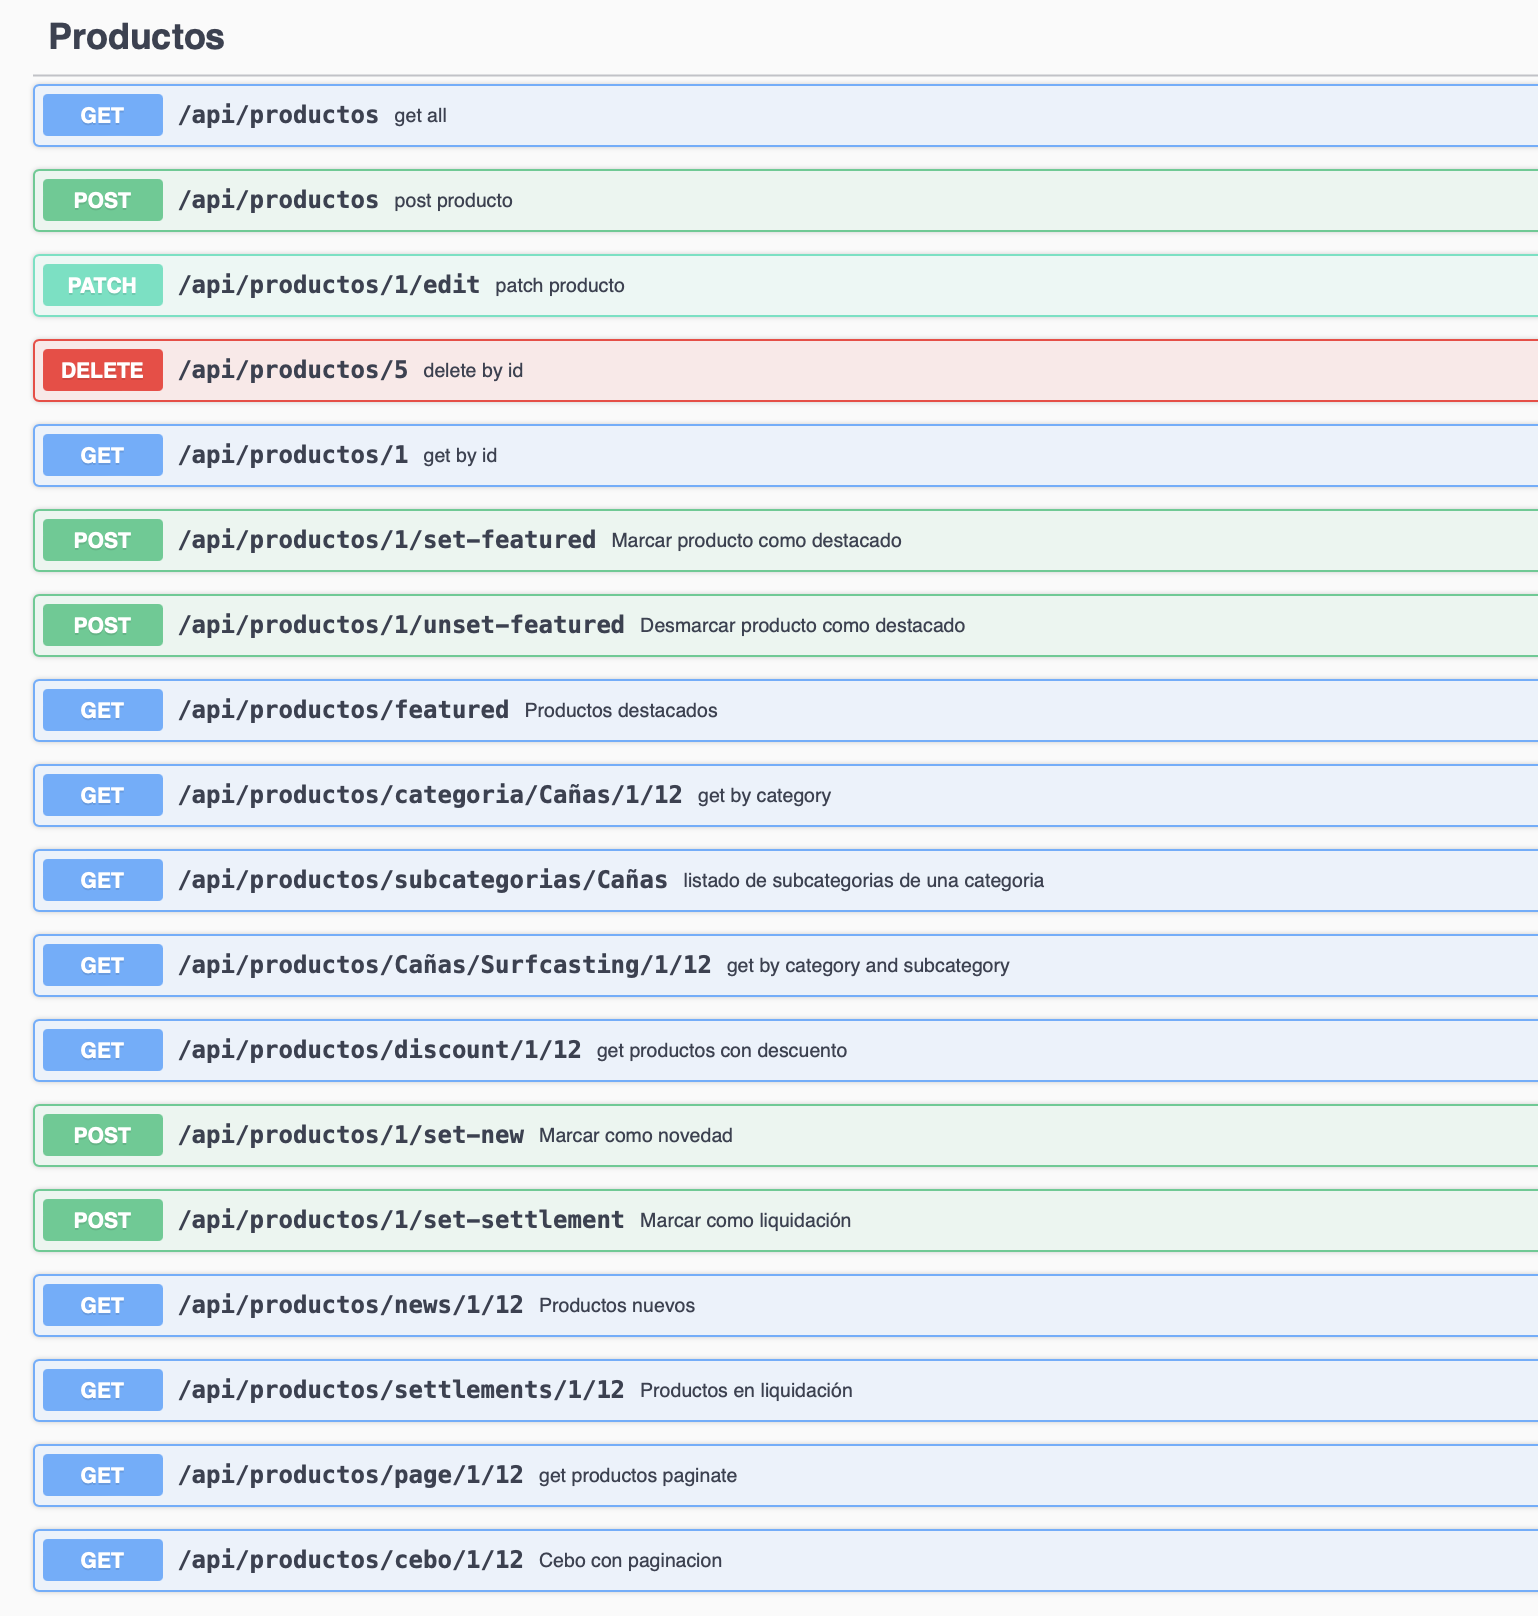
\includegraphics[scale=0.6]{./Images/APIproductos.png}
\caption{APIs de productos} Fuente: Elaboración propia.

\label{fig:fig1}

\end{center}
\end{figure}

\begin{figure}[H]
\begin{center}
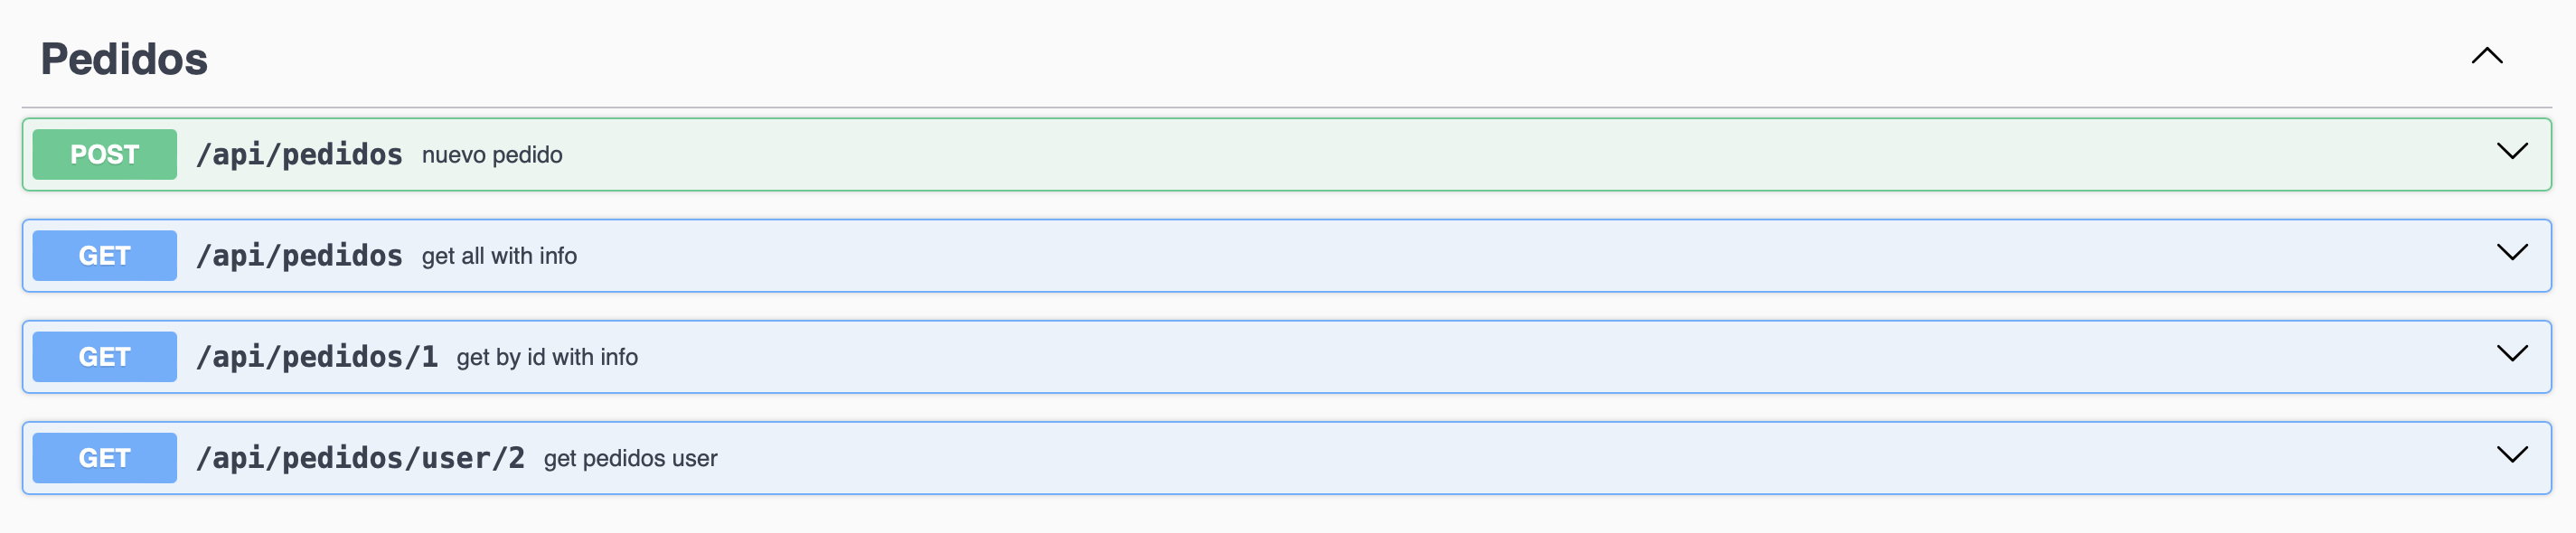
\includegraphics[scale=0.7]{./Images/APIpedidos.png}
\caption{APIs de pedidos} Fuente: Elaboración propia.

\label{fig:fig2}

\end{center}
\end{figure}

\begin{figure}[H]
\begin{center}
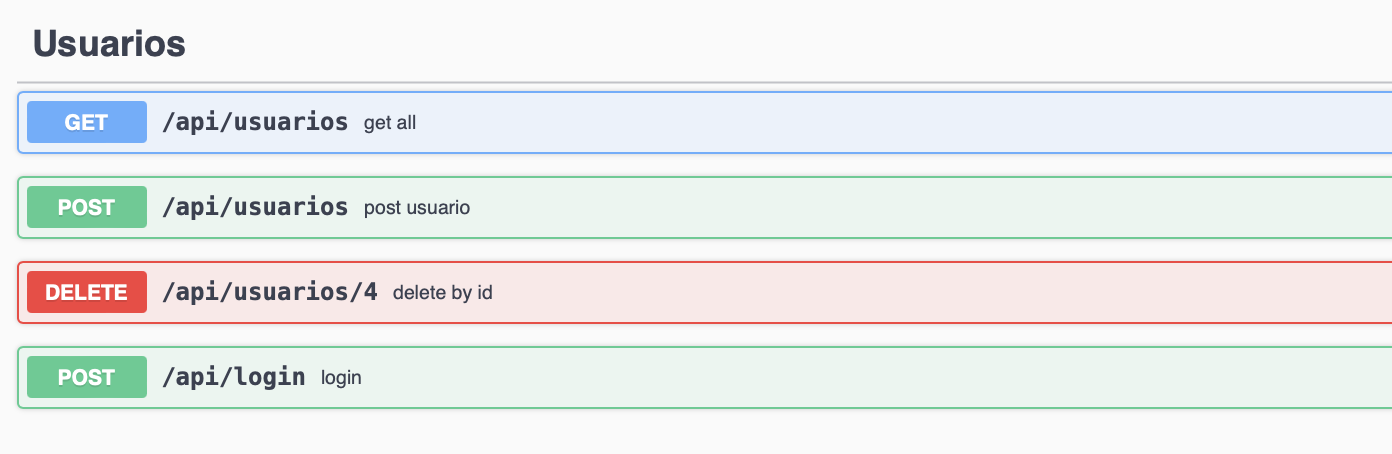
\includegraphics[scale=0.7]{./Images/APIusuarios.png}
\caption{APIs de usuarios} Fuente: Elaboración propia.

\label{fig:fig3}

\end{center}
\end{figure}

\begin{figure}[H]
\begin{center}
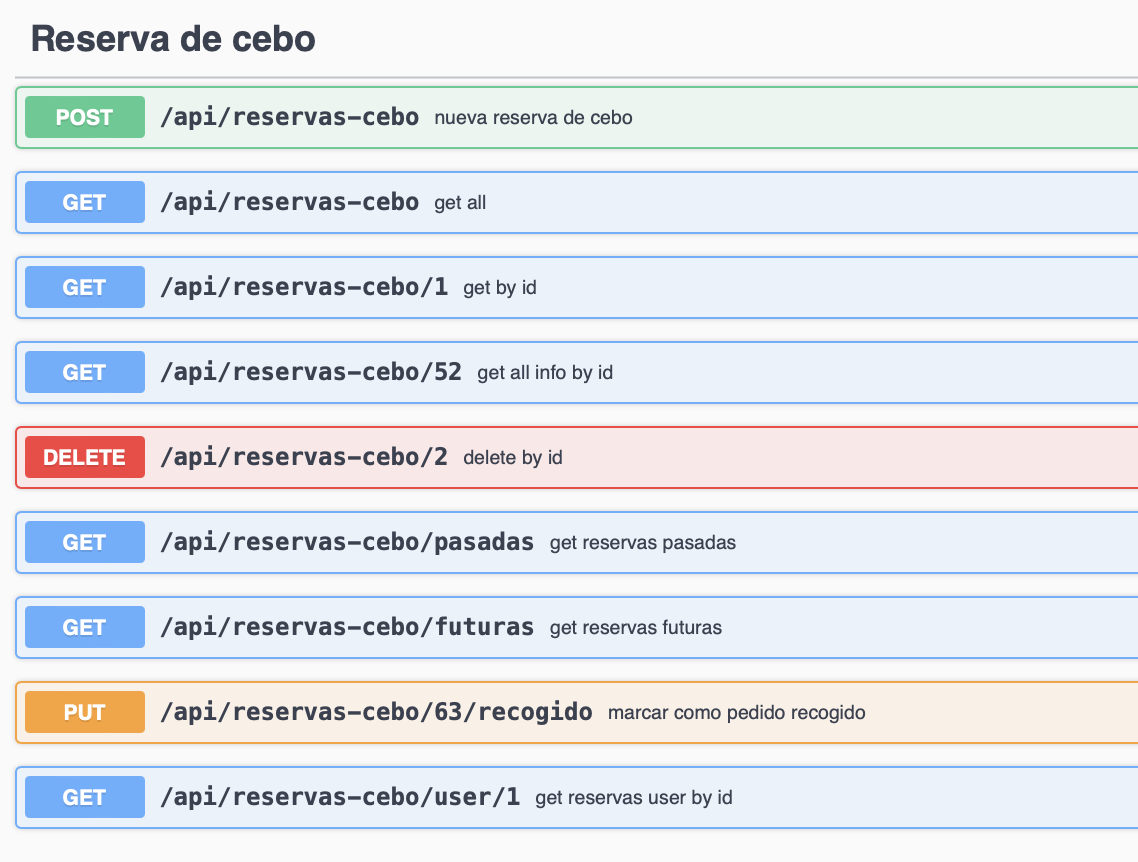
\includegraphics[scale=0.7]{./Images/APIreservacebo.png}
\caption{APIs de reserva de cebo} Fuente: Elaboración propia.

\label{fig:fig4}

\end{center}
\end{figure}

\begin{figure}[H]
\begin{center}
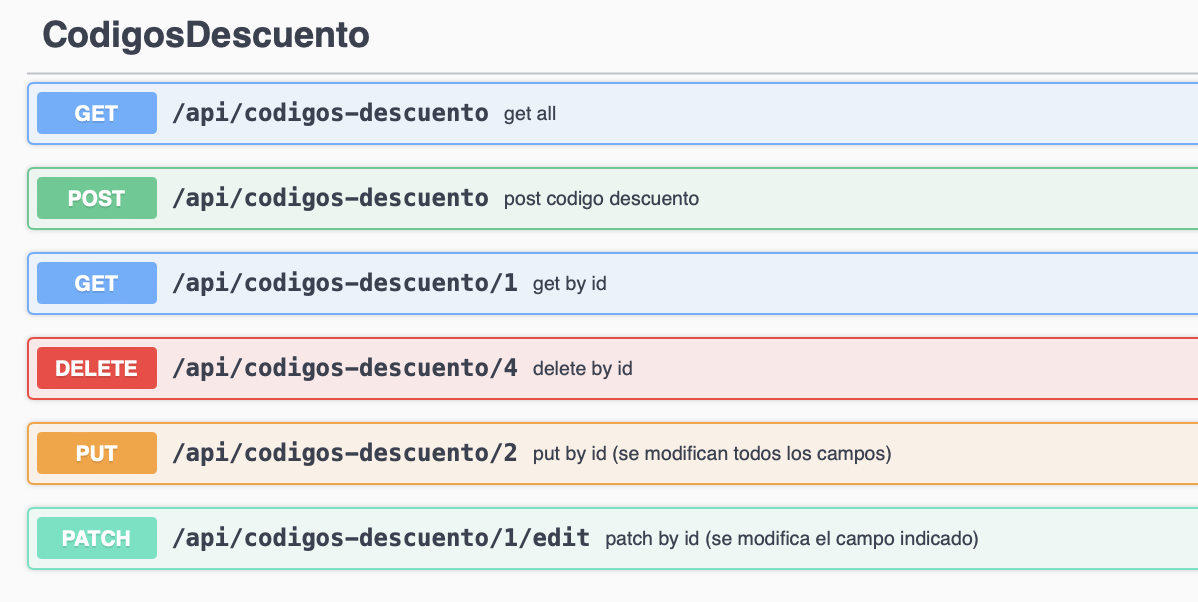
\includegraphics[scale=0.7]{./Images/APIcodigodescuento.png}
\caption{APIs de código de descuento} Fuente: Elaboración propia.

\label{fig:fig5}

\end{center}
\end{figure}

\begin{figure}[H]
\begin{center}
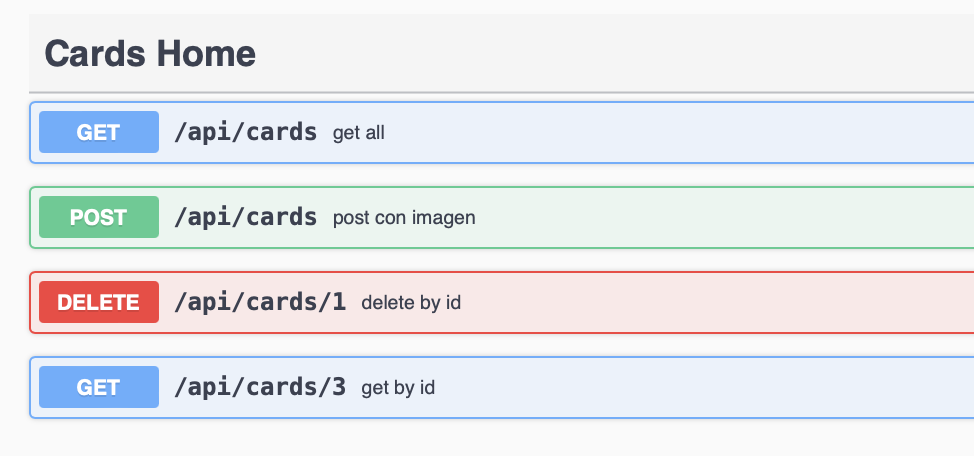
\includegraphics[scale=0.8]{./Images/APIcardshome.png}
\caption{APIs de cards de la home} Fuente: Elaboración propia.

\label{fig:fig6}

\end{center}
\end{figure}

\begin{figure}[H]
\begin{center}
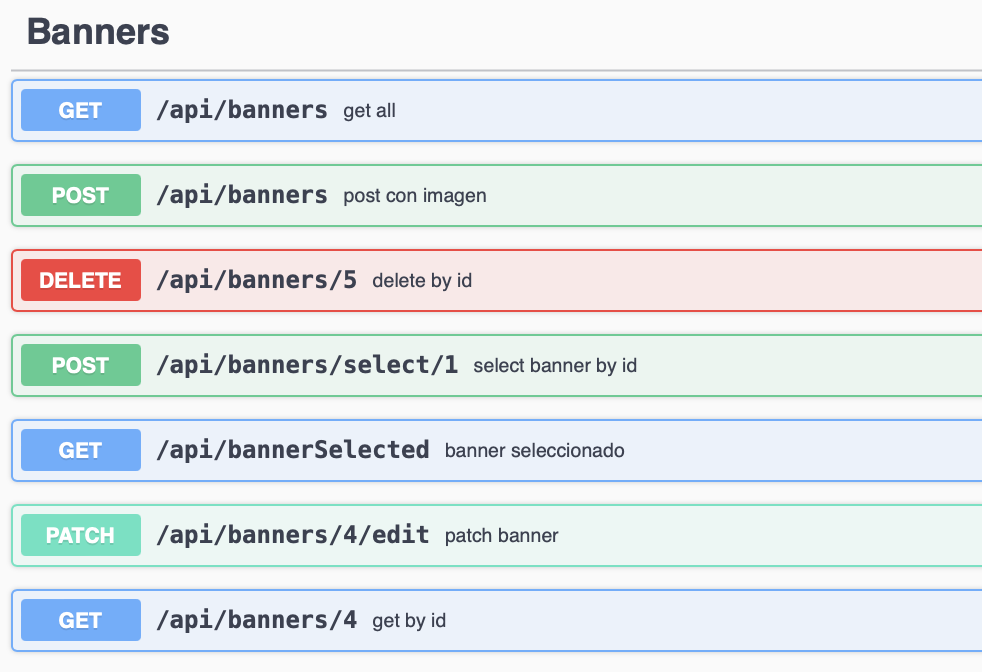
\includegraphics[scale=0.8]{./Images/APIbanners.png}
\caption{APIs banners} Fuente: Elaboración propia.

\label{fig:fig7}

\end{center}
\end{figure}

\begin{figure}[H]
\begin{center}
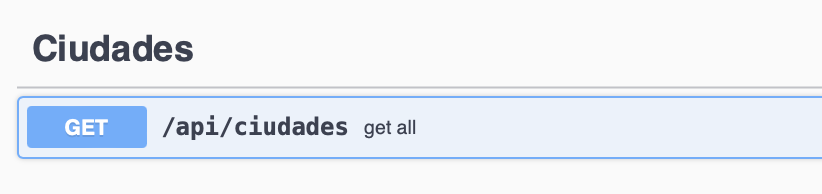
\includegraphics[scale=0.9]{./Images/APIciudades.png}
\caption{API ciudades} Fuente: Elaboración propia.

\label{fig:fig8}

\end{center}
\end{figure}

\begin{figure}[H]
\begin{center}
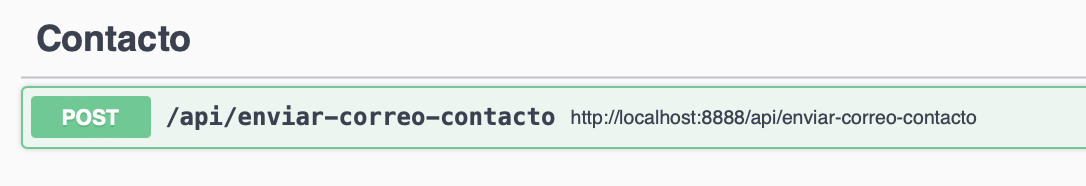
\includegraphics[scale=0.8]{./Images/APIcontacto.png}
\caption{API contacta con nosotros} Fuente: Elaboración propia.

\label{fig:fig9}

\end{center}
\end{figure}